\section{はじめに}

インターネット上の情報は利用する目的や形態から\textgt{フロー情報}と\textgt{ストック情報}の2つに分類できる.

\subsection*{フロー情報}

SNS,ニュース,IoT機器などリアルタイムに更新される情報.

\subsection*{ストック情報}

辞書,公式サイト,論文などいつでも参照できる情報.\vspace{0.2in}

現在のインターネットには特にフロー情報が溢れており,それらを情報の鮮度が落ちないうちに見ることができるインタフェースが求められている.

フロー情報を視覚化する手法として\textgt{ダッシュボード}(図\ref{dashing})がある.
ダッシュボードとは単一の画面に複数の情報をタイル状に並べて表示するもの\cite{few2005}で,センサの値や株価などのフロー情報をひと目で把握するのに非常に便利である.
ダッシュボードには様々な製品やサービスが存在し,多くの組織の壁掛けのディスプレイやデジタルサイネージで利用されている.
しかし,フロー情報のひとつである「人間の感情や現在の状況」というものをダッシュボードに表示することは行われてこなかった.
人間の感情や現在の状況をアウトプットする場としてSNSが利用されているが,数文字程度を表示するのが限度のダッシュボードのセルに表示するには適していない.
人間の感情や現在の状況をダッシュボードに表示するのに適した形でアウトプットできれば,タイムラインよりも遥かに効率良く,
大勢の人間の感情や現在の状況をひと目でチェックできるとのではないかと考えた.

本論文では,一般的にダッシュボードに表示される情報に加えて,人間の感情や現在の状況をスタンプで表現し表示することによって,
ありとあらゆるフロー情報を単一の画面に表示できる視覚化システム「\textgt{わかるらんど}」について述べる.

\begin{figure}[h]
\centering
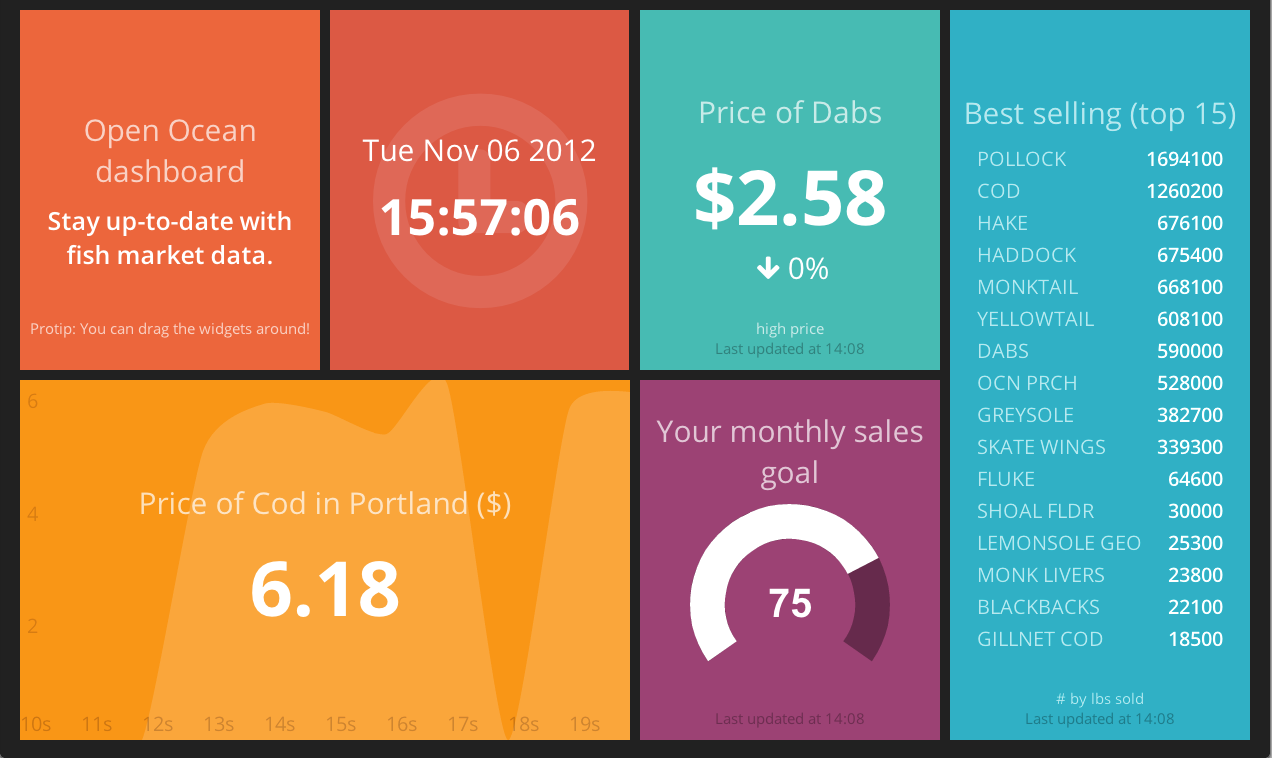
\includegraphics[width=7cm]{images/dashing.png}
\caption{Dashingによって作成されたダッシュボード}
\label{dashing}
\end{figure}